\documentclass{article} % For LaTeX2e
\usepackage[backend=bibtex, sorting=none]{biblatex}
\addbibresource{bibliography.bib}
\usepackage{nips15submit_e,times}
\usepackage{hyperref}
\usepackage{url}
\usepackage{amsmath}
\usepackage{tipa}
\usepackage{multicol}
\usepackage{multirow}
\usepackage{array}
\usepackage{graphicx}
\usepackage{bm}
\usepackage{mathtools,xparse}
\graphicspath{ {figures/} }
\newcolumntype{P}[1]{>{\centering\arraybackslash}p{#1}}
\usepackage[linesnumberedhidden,ruled,noend]{algorithm2e}

\makeatletter
\def\BState{\State\hskip-\ALG@thistlm}
\makeatother
%\documentstyle[nips14submit_09,times,art10]{article} % For LaTeX 2.09

\title{COMPM083: Statistical Natural Language Processing - Assignment 3}

\author{
Sergiu Tripon\\
Department of Computer Science\\
University College London\\
Gower Street, London, WC1E\\
\texttt{sergiu.tripon.15@ucl.ac.uk}\\
\And
Santiago Gonzalez\\
Department of Computer Science\\
University College London\\
Gower Street, London, WC1E\\
\texttt{hernan.toral.15@ucl.ac.uk} \\
\And
Archie Norman \\
Department of Computer Science\\
University College London\\
Gower Street, London, WC1E\\
\texttt{archie.norman.15@ucl.ac.uk} \\
}

% The \author macro works with any number of authors. There are two commands
% used to separate the names and addresses of multiple authors: \And and \AND.
%
% Using \And between authors leaves it to \LaTeX{} to determine where to break
% the lines. Using \AND forces a linebreak at that point. So, if \LaTeX{}
% puts 3 of 4 authors names on the first line, and the last on the second
% line, try using \AND instead of \And before the third author name.

\newcommand{\fix}{\marginpar{FIX}}
\newcommand{\new}{\marginpar{NEW}}

\nipsfinalcopy % Uncomment for camera-ready version

\begin{document}

\maketitle

\section{Problem 1: Gradient Checking}

Gradient checking is a good approach to test the gradient of a model and/or the possible activation functions to be used in, but even if we measure it to an arbitrary precision it cannot be used to train our model instead of developing a proper backpropagation algorithm. While speaking about efficiency, the Gradient Check evaluates the activation function (or model\ i.e the loss function twice to check every single dimension of the gradient, being a second order approximation error $O(\epsilon^2)$. On the other hand, when running the Gradient Check, it performs at a random point in the space of parameters. Even if the test succeeds at that point, within a given small error window, it is not certain that the gradient approximation will give a correct implementation globally.\cite{StandfordUniversity} Table \ref{table:averageError} shows the obtained average deviation by executing the Gradient Check on two of the implemented models of the assignment using 10 neurons and a regularization parameter of 1 (in order to make the regularizer function as visible as possible).

\begin{table}[!htp]
\caption{Average deviation from the approximated gradient for the 2 implemented models.}
\label{table:averageError}
\begin{center}
\begin{tabular}{c c c}
\multicolumn{1}{c}{} & \multicolumn{2}{c}{\bf Models}
\\ \hline \\
{} & \textbf{SumOf-Word-Vectors} & \textbf{RNN}\\
\textit{Average error} & $7.93E^{-10}$ & $9.59E^{-10}$ \\
\end{tabular}
\end{center}
\end{table}

\section{Problem 2: Sum-of-Word-Vectors Model}

\subsection{Gradient Blocks}

\subsubsection*{Dot Product}

\begin{equation}
z\frac{\partial \bm{x} \cdot \bm{y}}{\partial \bm{x}} = z\bm{y}
\qquad
z\frac{\partial \bm{x} \cdot \bm{y}}{\partial \bm{y}} = z\bm{x}
\end{equation}

\subsubsection*{Sigmoid}

\begin{equation}
z\frac{\partial sigmoid(x)}{\partial x} = sigmoid(x) \cdot (1-sigmoid(x))
\end{equation}

\subsubsection*{Negative Log-Likelihood}

\begin{equation}
\frac{\partial \mathcal{L}(f(x),y)}{\partial f(x)} = \frac{y-f(x)}{f(x)\cdot(f(x)-1)}
\end{equation}

\subsubsection*{$\ell_2$ Regularization}

\DeclarePairedDelimiter{\norm}{\lVert}{\rVert}

\begin{equation}
\frac{\partial \lambda\frac{1}{2}\norm{\theta}_{2}^2}{\partial \theta} = \frac{\partial \lambda\frac{1}{2}\norm{\bm{\theta}^{T}\bm{\theta}}_{2}}{\partial \bm{\theta}} = \lambda\bm{\theta}
\end{equation}

\subsection{Model}

Table \ref{table:sumOfWords} shows the average error obtained by testing the whole the model using Gradient Check and a random example from the training set. Two test cases have been taken into account: a) a model with the highest value of regularization, and b) a model without the regularization term.

\begin{table}[!htp]
\caption{Difference on testing the Sum-Of-Word-Vectors Model with Gradient Checking.}
\label{table:sumOfWords}
\begin{center}
\begin{tabular}{c c}
\textbf{$\lambda=1$} & \textbf{$\lambda=0$}\\
\hline \\
$7.93E^{-10}$ & $8.13E^{-10}$ \\
\end{tabular}
\end{center}
\end{table}

\subsection{Grid Search and Evaluation}

\begin{table}[!htbp]
\caption{Evaluation results of the Sum-of-Word-Vectors Model on the dev set. Best configuration is shown in {\bf bold}.}
\label{table:GridSearchSWVM}
\begin{center}
\begin{tabular}{ P{1cm} P{1cm} P{1cm} P{2cm} P{1cm} P{2cm} P{1cm} P{1cm} }
\textbf{ID} & \textbf{Epoch} & \textbf{Word Dim} & \textbf{Reg. Strength} & \textbf{L Rate} & \textbf{Loss} & \textbf{Train Acc} & \textbf{Dev Acc}\\
\hline\\

1 & 73 & 10 & 0.01 & 0.001 & 39172.2081 & 92.04 & 77.16\\
2 & 61 & 10 & 0.01 & 0.002 & 30629.0345 & 96.48 & 77.16\\
\\

3 & 73 & 10 & 0.04 & 0.001 & 56484.8333 & 84.91 & 77.83\\
4 & 76 & 10 & 0.05 & 0.001 & 58780.4346 & 84.51 & 77.83\\
5 & 99 & 10 & 0.06 & 0.001 & 58443.3446 & 85.96 & 77.96\\
6 & 91 & 10 & 0.07 & 0.001 & 61507.1410 & 84.78 & 78.03\\
7 & 28 & 10 & 0.004 & 0.001 & 48806.5579 & 84.88 & 76.9\\
8 & 40 & 10 & 0.005 & 0.001 & 43265.8564 & 88.62 & 76.96\\
\\

9 & 95 & 8 & 0.07 & 0.01 & 60635.5750 & 85.27 & 76.5\\
10 & 97 & 9 & 0.07 & 0.01 & 60685.5176 & 85.25 & 77.36\\

\textbf{11} & \textbf{91} & \textbf{10} & \textbf{0.07} & \textbf{0.001} & \textbf{61507.1410} & \textbf{84.78} & \textbf{78.03}\\

12 & 95 & 11 & 0.07 & 0.01 & 61207.1211 & 85.16 & 77.36\\
13 & 87 & 12 & 0.07 & 0.01 & 62230.5593 & 84.64 & 77.43\\
\end{tabular}
\end{center}
\end{table}

A grid search was performed over the hyperparameters of the model. A number of results from this evaluation are shown in Table \ref{table:GridSearchSWVM} where the best configuration of the Sum-of-Word-Vectors Model is in \textbf{bold}. The default hyperparameters provided within the assignment code were: 0.01 (Learning Rate), 0.01 (Regularization Strength) and 10 (Dimension of Word Vectors). For each hyperparameter, a range of values were tested in order to identify the value that produces the best accuracy result.

All tests were performed using 100 as the epoch parameter. However, to identify the best accuracy results, the notion of regularization by "early stopping" was applied, which allowed us to identify and consider the best accuracy result at a specific epoch.

\subsection*{Learning rate (ID: 1-2)}

The first objective of the evaluation was to identify an ideal learning rate. For this, we used default values for regularization strength and dimension of word vectors. It was found that the default learning rate of 0.01 lead to exploding weights indicating that a lower learning rate was required. Then values between 0.001 and 0.02 were tested, where learning rates of 0.001 and 0.002 produced an identical best result on the dev set with an accuracy of 77.16\%. However, by using 0.002, the best result was produced more efficiently, within 62 epochs. Therefore, at the end of this evaluation, we established that the best configuration of the learning rate can be either 0.001 or 0.002, but as a result of the full grid search we conclude that the best configuration for learning rate is in fact 0.001.

\subsection*{Regularization strength (ID: 3-8)}

The second objective was to identify an ideal regularization strength. For this evaluation, we used the optimum learning rate identified previously and the default value for dimension of word vectors. During the tests, it was clear that a learning rate of 0.001 produced better results than 0.002. Regularization values ranging between 0.001 and 0.7 were used, and we found that a strength value of 0.07 produced the best accuracy result on the dev set with an accuracy of 78.03\%, within 92 epochs. Therefore, at the end of this evaluation, we established that the best configuration of the regularization strength is 0.07.

\subsection*{Dimension of word vectors (ID: 9-13)}

The third objective was to identify an ideal dimension of word vectors. For this evaluation, we used the optimum learning rate and regularization strength identified in the previous steps. Values ranging between 7 and 13 were tested, and it was found that the default dimension of word vectors (10) produced the best result with an accuracy on the dev set of 77.83\%, within 92 epochs. Therefore, at the end of this evaluation, we established that the best configuration of the dimension of word vectors is 10.

Finally, the evaluation carried out supports our conclusion that the best hyperparameter configuration, yielding the best accuracy results is as follows: 

\begin{itemize}
\item \textbf{Learning Rate} - 0.001
\item \textbf{Vector Regularization Strength} - 0.07
\item \textbf{Dimension of Word Vectors} - 10
\ldots
\end{itemize}

\subsection{Loss Analysis}

Sara et. al. \cite{silva2010measuring} states "that the best model is the one that minimizes the amount of information needed to encode it. Simpler solutions are thought to be more robust and generalize better, while complex solutions are more likely to incorporate specific information from the training set, thus overfitting it." From this, we can say that underfitting occurs when the model cannot minimize the amount of information needed to encode it. On the other hand, in the bias-variance approach, when the model underfits it means that the model is experiencing high bias and when the model overfits  the model has high variance.

The loss analysis can provide an indication of whether the model suffers from overfitting or underfitting. Figure \ref{fig:LossAnalysisSWVM1} shows the loss within the Sum-of-Word-Vectors Model, while Figure \ref{fig:LossAnalysisSWVM2} shows the train and dev accuracy within the Sum-of-Word-Vectors Model by recording a test case using 100 epochs. By making an analysis between the training set loss and the training set accuracy we can see that mainly, they both decrease and increase respectively. The loss got lower on each timestep, while the accuracy improved. This indicates that the model performed well on the training set. even though between epoch 40 and 80, we can see that the increasing accuracy fluctuated slightly, stating a possible evidence of symptoms of overfitting within the model.

However, while analysing the model accuracy on the dev set, it is clear from the start that the model suffers from overfitting. The dev set accuracy increases gradually during the first 10 epochs, much like the train set accuracy, but it then starts to fluctuate heavily throughout, all the way to the end.

\begin{figure}[!htbp]
\centering
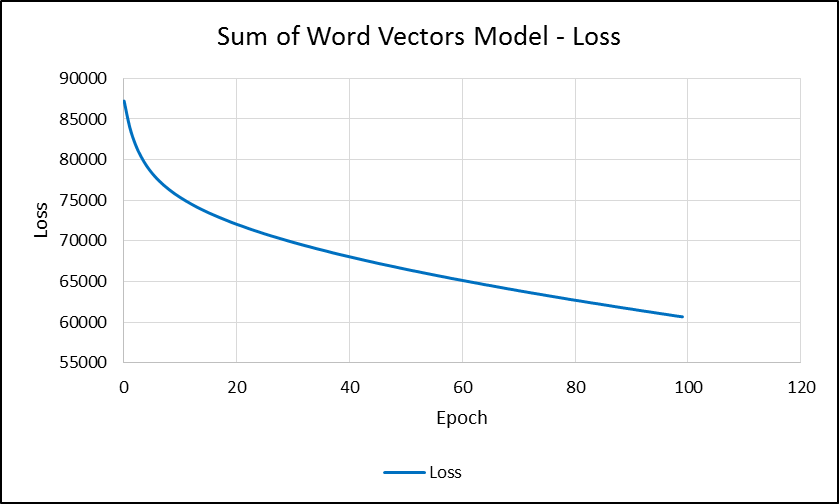
\includegraphics{Loss}
\caption{Loss within the Sum-of-Word-Vectors Model during 100 epochs on the dev set.}
\label{fig:LossAnalysisSWVM1}
\end{figure}

\begin{figure}[!htbp]
\centering
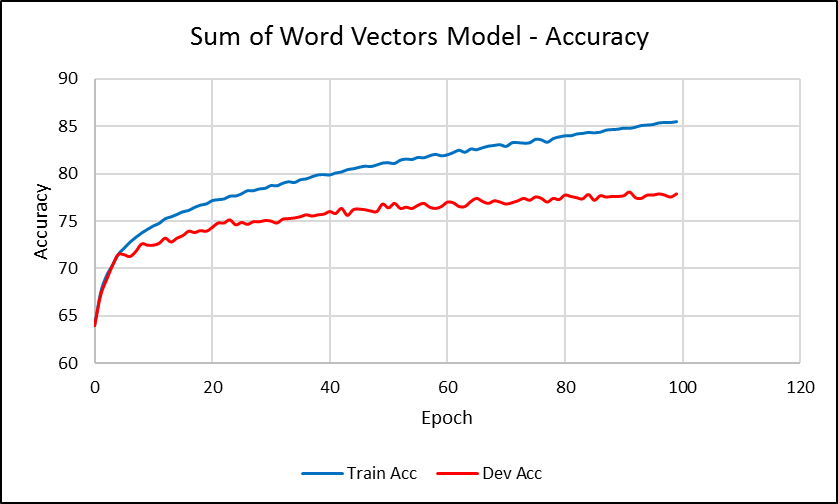
\includegraphics{Accuracy}
\caption{Accuracy within the Sum-of-Word-Vectors Model during 100 epochs on the dev set.}
\label{fig:LossAnalysisSWVM2}
\end{figure}

\subsection{t-SNE Visualization}

We used the t-SNE algorithm\cite{van2008visualizing} to reduce the number of dimensions given in the model output to a two dimensional space, as shown in Figure \ref{fig:tsne}. This results in a scatter plot indicating word clusters consisting of similar objects while different objects are positioned further away from each other. The figure shows two high scoring words contributing to negative tweets, 'shitty' scored 0.245812514478475 and 'good-bye' 0.268014130338353. Positive words included 'Welcome' scoring 0.762748299508867 and 'hehe' scored 0.726878049879343. These high scoring words were found in the sample of one thousand words used in this plot.

\begin{figure}[!htbp]
\centering
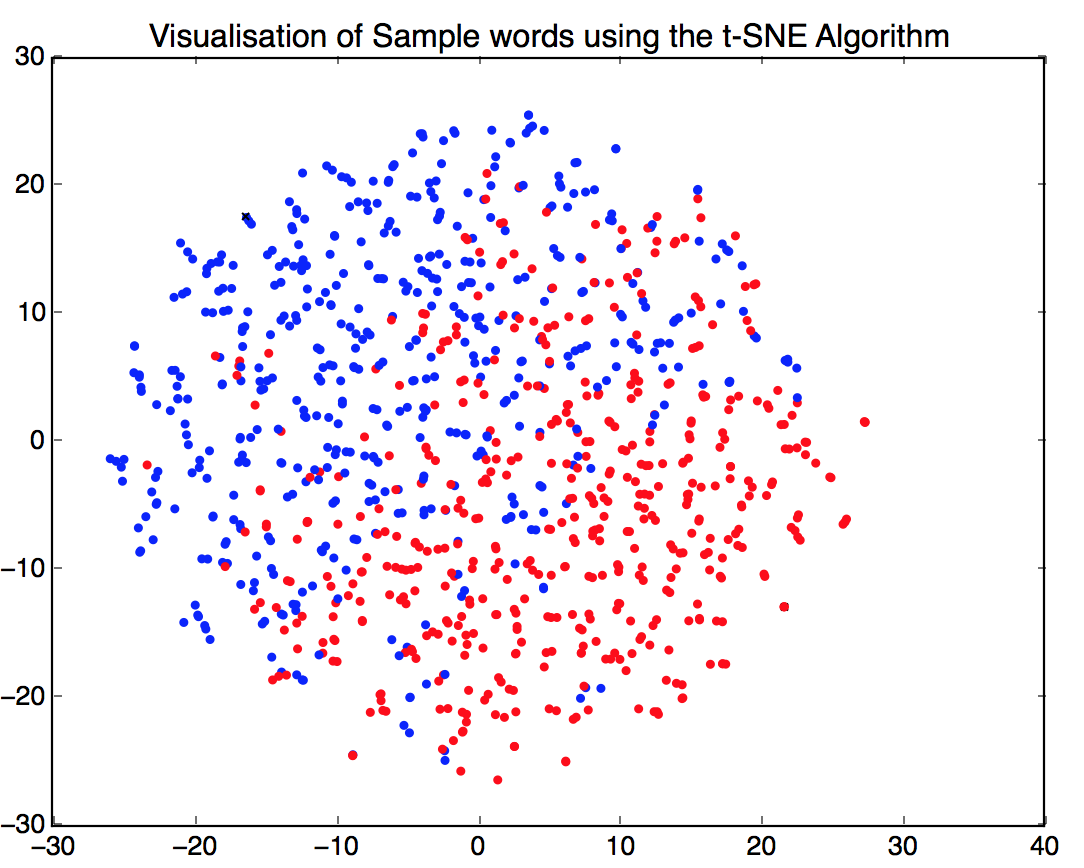
\includegraphics[scale=0.75]{tsne}
\caption{Shows a visualisation of positive and negative words represented as a scatter graph.}
\label{fig:tsne}
\end{figure}

\section{Problem 3: Recurrent Neural Networks}

\subsection{Gradient Blocks}

\subsubsection*{Matrix-Vector Multiplication}

\begin{equation}
z\frac{\partial \bm{W} \cdot \bm{x}}{\partial \bm{x}} = z\bm{W^T}
\qquad
z\frac{\partial \bm{W} \cdot \bm{x}}{\partial \bm{W}} = z\bm{x^T}
\end{equation}

\subsubsection*{Tanh}

\begin{equation}
\bm{z}\frac{\partial tanh(\bm{x})}{\partial \bm{x}} = \frac{1}{cosh^2(\bm{x})}
\end{equation}

\subsection{Model}

Table \ref{table:rnn} shows the average error obtained by testing the whole the model using Gradient Check and a random example from the training set. Two test cases have been taken into account: a) a model with the highest value of regularization, and b) a model without the regularization term.

\begin{table}[!htp]
\caption{Average deviation from the approximated gradient for the 2 implemented models.}
\label{table:rnn}
\begin{center}
\begin{tabular}{c c}
\textbf{$\lambda=1$} & \textbf{$\lambda=0$}\\
\hline \\
$9.59E^{-10}$ & $0$\\
\end{tabular}
\end{center}
\end{table}

\subsection{Grid Search, Initialization, Evaluation and Comparison}

\begin{table}[!htbp]
\caption{Evaluation results of the Recurrent Neural Network Model on the dev set. Best configuration is shown in {\bf bold}.}
\label{table:GridSearchRNNM}
\begin{center}
\begin{tabular}{ P{0.3cm} P{0.8cm} P{0.8cm} P{0.8cm} P{1.2cm} P{1.2cm} P{1cm} P{1.5cm} P{1cm} P{1cm} }
\textbf{ID} & \textbf{Epoch} & \textbf{Word Dim} & \textbf{Hidden Dim} & \textbf{(V) Reg. Strength} & \textbf{(M) Reg. Strength} & \textbf{L Rate} & \textbf{Loss} & \textbf{Train Acc} & \textbf{Dev Acc}\\
\hline\\

\textbf{1} & \textbf{5} & \textbf{10} & \textbf{10} & \textbf{0.02} & \textbf{0.0} & \textbf{0.01} & \textbf{71328.4682} & \textbf{73.02} & \textbf{70.57}\\
2 & 5 & 10 & 10 & 0.03 & 0.0 & 0.01 & 73392.8655 & 71.29 & 69.91\\
3 & 5 & 10 & 10 & 0.01 & 0.0 & 0.01 & 69338.7099 & 74.99 & 69.24\\

\\

4 & 5 & 10 & 10 & 0.01 & 0.0 & 0.02 & 64562.1742 & 78.75 & 69.17\\
5 & 3 & 10 & 10 & 0.02 & 0.0 & 0.02 & 76264.7173 & 70.91 & 68.58\\

\\

6 & 5 & 10 & 10 & 0.01 & 0.0 & 0.01 & 71325.9495 & 73.00 & 68.44\\
\end{tabular}
\end{center}
\end{table}

First of all, it is important to mention that prior to the grid search, the Recurrent Neural Network Model, using default configuration, produced an accuracy on the dev set of 68.44\% (ID 6) during its first dry run.
After that, a small grid search was performed over the hyperparameters of the model. The results obtained from this evaluation are shown in Table \ref{table:GridSearchRNNM}. The best configuration for the RNN model is shown in \textbf{bold}. The default hyperparameters provided within the assignment code were: 0.01 (Learning Rate), 0.01 (Vector Regularization Strength), 0.0 (Matrix Regularization Strength), 10 (Dimension of Word Vectors), 10 (Hidden dimension). Finally, for each hyperparameter, a range of values were tested in order to identify the value that produces the best accuracy result.

All tests were performed using 50 (0-50) as the epoch parameter. However, to identify the best accuracy results, the notion of regularization by "early stopping" was applied, which allowed us to identify and consider the best accuracy result at a specific epoch.

Furthermore, besides the provided default weight initialization, a generalization using the "xavier" weight initialization \cite{Glorot2010} \cite{he2015delving} was also implemented and tested. In that way we could change the values for the hidden dimensions withouth affecting the fact that the Matrix initilization should be generated by a random distribution with variance=1 and mean=0. In Table \ref{table:GridSearchRNNM}, IDs 1-3 represent results produced using the "xavier" weight initialization, while IDs 4-5 represent results produced using the default weight initialization. As can be seen, using the "xavier" weight initialization resulted in the best dev accuracy result, with a 70.57\%.

\subsection*{Learning Rate}

The first objective of the evaluation was to identify an ideal learning rate. For this evaluation, we used default values for the other hyperparameters. Values ranging between 0.01 and 0.05 were tested, and it was found that the learning rate of 0.02 produced the best result, with an accuracy of 69.17\% (on the dev set) within 5 epochs. At the end of this evaluation, we established that the best configuration of the learning rate is 0.02 but later on as a result of the regularization strength tests, we conclude that the best configuration of the learning rate is in fact, 0.01. Subsequently, as a result of the Vector Regularization Strength evaluation, we conclude that the best configuration of the learning rate is in fact, 0.01.

\subsection*{Regularization Strength (Vector \& Matrix)}

The second objective was to identify the ideal vector and matrix regularization strengths. For this evaluation, we used the optimum learning rate identified and default values for the other hyperparameters. Values ranging between 0.01 and 0.1 were tested for both regularization strength parameters. A vector regularization strength of 0.02 was identified as best, which produced the best accuracy result with 70.57\% within 5 epochs. However, matrix regularization strength values other than the default 0.0 caused accuracy results to drop radically. This is the case for both default and xavier weight initialization. We believe this is due to the way the matrix weights are initialized. Therefore, at the end of this evaluation, we established the best configuration of the vector regularization strength is 0.02, but haven't established a best configuration for the matrix regularization strength.

\subsection*{Dimension of word vectors \& Hidden dimension}

The third objective was to identify an ideal dimension of word vectors and hidden dimension. For this evaluation, we used the optimum learning rate and vector regularization strength identified previously. Values ranging between 8 and 12 were tested for both dimensions, and it was found that a dimension of word vectors of 10 and hidden dimension of 10 produced the best result, with a 70.57\% accuracy, within 5 epochs. Therefore, at the end of evaluation, we established that the best configuration of the dimension of word vectors and hidden dimension is 10.

Finally, we believe that the evaluation carried out supports our conclusion that the best hyperparameter configuration, yielding the best accuracy results is as follows: 
\begin{itemize}
\item \textbf{Learning Rate} - 0.01
\item \textbf{Vector Regularization Strength} - 0.02
\item \textbf{Matrix Regularization Strength} - 0.0
\item \textbf{Dimension of Word Vectors} - 10
\item \textbf{Hidden Dimension} - 10
\item \textbf{Initialization of Weights} - "xavier" initialization
\end{itemize}

\subsection*{Comparison to Sum-of-Word-Vectors Model}

The best dev set accuracy result of the Sum-of-Word-Vectors Model was 78.03\%, while the best dev set accuracy results of the Recurrent Neural Network Model was 70.57\%, which shows that the latter performed worse on the dev set. The best result of the Sum-of-Word-Vectors Model was produced within 91 epochs, compared to the best result of the Recurrent Neural Network which was produced within 5 epochs. This is the case because of a number of potential reasons. Firstly, the grid search conducted for the Recurrent Neural Network Model was smaller but a larger grid search could potentially produce a better accuracy result. Secondly, there are more weight initialization methods that can be implemented, which could further improve the accuracy result. Thirdly, training the standard RNN model can be time-consuming and problematic \cite{pascanu2012difficulty} because of its slow learning nature. Better alternatives exist such as LSTM or GRU. Finally, we believe that implementing additional blocks in order to tackle issues such as overfitting will produce an accuracy result much closer to the result produced by the Sum-of-Word-Vectors Model.

\section{Problem 4: Sky's the Limit}

\subsection{Approaches for a better model}

In a standard Recurrent Neural Network, during back-propagation, the gradient signal ends up being multiplied a large number of times by the weight matrix associated with the connections between the neurons of the recurrent hidden layer, which has a strong impact on the learning process. Due to the weights in the matrix becoming smaller, it leads to an event called \textit{vanishing gradients} where the gradient signal gets so small that the learning process either becomes very slow, stops working and/or causes overfitting. In the following sections, we present different approaches we implemented in order to produce a better model that performs best on the test set. However, due to the nature of the architecture we are using, performance issues cannot be resolved, and we conclude that a more distributed model should be taken into account when implementing RNN models (e.g. the \textit{theano} library uses mini batches to process the RNN models efficiently).

\subsubsection*{word2vec}

As one of our modeling choices, we chose to load pre-trained vectors using \textit{word2vec}. It "provides an efficient implementation of the continuous bag-of-words and skip-gram architectures for computing vector representations of words."\cite{word2vec} word2vec seeks to identify similarities between words in a mathematical way using their vector representations. Subsequently, it groups the vector representations into vector space. As a result of this, word2vec is able to make high accuracy predictions in regards to what a word means, based on its past occurrences. Therefore, using these predictions we are able to build relationships with other words and produce more accurate sentiment predictions.

In practice, word2vec takes a text corpus as input and outputs a set of vectors. In this context, the "vocab.tsv" file was the used as input. This file contains a vocabulary of all the words within the tweets. The word2vec output is the "vectors.txt" file.\footnote{word2vec output file download link: \url{http://bit.ly/1NLQ95U}}. This file consists of the words in the vocabulary and their vector representation. Vector representations were produced for all vocabulary words. Each word was turned into a vector representation of size 10.

Furthermore, an extra method called \textit{loadFixedWordVectors} was implemented on the Model trait to allow the insertion of this pre-trained word vectors on any of the models built.

\subsubsection*{Dropout}

Another modeling choice was to implement the Dropout block provided in the assignment code. Dropout is a widely used technique that helps to reduce the overfitting we may experience and provides an efficient way to combine different neural networks configurations. In order to implement the we had to randomly remove units (using the Bernoulli distribution to drop incoming and outgoing connections) from the network and thus obtain a "thinned" network for each time step during training. "At test time, it is easy to approximate the effect of averaging the predictions of all these thinned networks by simply using a single unthinned network that has smaller weights".\cite{Srivastava2014}

\subsubsection*{Recurrent Neural Network - LSTM}

As a second approach for a better model, we implemented a version of the LSTM model which introduces a new structure called a memory cell. It is composed of four main elements: a) \textit{an input gate} that allows/block incoming signal to alter the state of the memory cell; b) \textit{a neuron with a self-recurrent connection} ensures that the state of a memory cell can remain constant from one timestep to another; c) \textit{a forget gate} modulates the memory cell’s self-recurrent connection, allowing it to remember or forget its previous state, as needed; and d) \textit{an output gate} that allow/prevent the state of the memory cell to have an effect on other neurons. In brief, the main reason LSTM should perform better is that during the recurrency, the activation function is an identity function with derivative of 1.0, so the backpropagated gradient neither vanishes or explodes when passing through, but remains constant.

In order to build this model, we had to implement two extra blocks: the Multiplication-of-Word-Vectors model and the Element-wise sigmoid.Additionally, we use LSTM in conjunction with Dropout to try to get the best possible results. It is important to mention that we experienced performance issues by using this model due to it process \textit{n} times the number of calculations performed in a standard RNN configuration per gate that the LSTM model has. It has to be computed in that manner because of the block nature of our implementation. However, one approach to improve this in a different architecture, is to zip all the weight matrices and biases as a superset and compute the results in one run. At the end, a split procedure can be done to finally get the final sentence representation that will be used by the classifier.

\subsection*{Best Model and Results}

For our best model, we use we a combination of LSTM and Dropout. Additionally, we included the word vectors obtained by running the \textit{word2vec} tool as the initial weights for training. Due to the bad performance of the implemented model in a non-distributed environment, we could not execute a full grid search to find the ideal hyperparameters in order to get the best accuracy on the test set by using the train set for training. For fastest tests purposes, we tested each module (word2vec and Dropout) separately, which resulted in better accuracy values than the standard RNN accuracy we got initially. Finally, by changing the hyperparameters values \textit{learningRate = 0.001 vectorRegularizationStrength = 0.07} in comparison to the default configuration of the assignment, we obtained our best accuracy of 80.78\% on the test set.

\printbibliography
\end{document}